\documentclass{article}
\usepackage[spanish, es-tabla]{babel}

\usepackage{amsmath}
\usepackage{amssymb}
\usepackage{amsthm}
\usepackage{booktabs}
\usepackage{bigstrut}

\usepackage{fontspec}
\usepackage{multicol}
\usepackage{graphicx}
\usepackage{float}
\usepackage[center]{caption}
\usepackage{graphicx}
\usepackage{listings}
\usepackage[dvipsnames, table]{xcolor}
\usepackage{multirow}
\usepackage{fancyhdr}
\usepackage{pdfpages}
\usepackage{titling}
\usepackage[fixlanguage]{babelbib}
\selectbiblanguage{spanish}
\usepackage{subcaption}
\captionsetup{labelfont=bf}
% \captionsetup[table]{labelfont={bf},name={Tabla},labelsep=period}
\usepackage{hyperref}
\definecolor{blueX}{HTML}{3f84e4}
\setmonofont{SFMonoRegular.otf}
\usepackage[margin=2.8cm]{geometry}
\hypersetup{
    colorlinks,
    citecolor=black,
    filecolor=black,
    linkcolor=black,
    urlcolor=black
}
\usepackage{siunitx}
\sisetup{
    per-mode = fraction,
    detect-all,
    exponent-product = \cdot
}
\usepackage{enumitem}
\usepackage{pdflscape}
\usepackage[stylemods,style=super, nogroupskip, toc=false, hyperfirst=false, nonumberlist]{glossaries-extra}

\setlength{\parindent}{0pt} % To avoid indentation
\setabbreviationstyle[acronym]{long-short}
\makenoidxglossaries
\newglossary{difusion}{difusionin}{difusionout}{Glosario}
\loadglsentries{glosario}

% COLUMNAS Y FILAS MULTIPLES DENTRO DE TABLAS
\usepackage{multirow, hhline}
\usepackage{array}
\newcolumntype{L}[1]{>{\raggedright\let\newline\\\arraybackslash\hspace{0pt}}m{#1}}
\newcolumntype{C}[1]{>{\centering\let\newline\\\arraybackslash\hspace{0pt}}m{#1}}
\newcolumntype{R}[1]{>{\raggedleft\let\newline\\\arraybackslash\hspace{0pt}}m{#1}}
\renewcommand{\listfigurename}{Figuras}
\renewcommand{\listtablename}{Tablas}

\renewcommand{\familydefault}{\sfdefault}
\renewcommand{\thesubsubsection}{\alph{subsubsection}}

\usepackage{titlesec}
\titleformat*{\subsection}{\normalsize\bfseries}
\titleformat*{\subsubsection}{\normalsize\bfseries}

\titlespacing\subsection{0pt}{12pt plus 4pt minus 2pt}{0pt plus 2pt minus 2pt}
\titlespacing\subsubsection{0pt}{12pt plus 4pt minus 2pt}{0pt plus 2pt minus 2pt}

\begin{document}

\title{\textbf{Práctica 3\\Refuerzo sonoro de una sala}}
\author{Javier Rodrigo López}
\date{\today}
\maketitle

\pagenumbering{gobble}

\fancypagestyle{firststyle}
{
    \fancyhead[L]{Sistemas Electroacústicos}
    \fancyhead[R]{
\includegraphics[width=0.3\linewidth]{Imágenes/ETSIST.png}}
    %\fancyfoot[R]{
\includegraphics[width=0.08\linewidth]{Imágenes/Plantilla_IAC.png}\\Departamento de Ingeniería Audiovisual y Comunicaciones}
}

\thispagestyle{firststyle}

% \newpage

\fancyhead{}
\pagestyle{fancy}

\pagestyle{fancy}
\fancyhead[L]{Difusión de Contenidos Audiovisuales}
\fancyhead[R]{Curso 2023/24}

%\newpage
%\tableofcontents
%\listoffigures
\setcounter{figure}{0}
\setlength{\parskip}{0.5em}

\hypersetup{
    citecolor=black,
    filecolor=black,
    linkcolor=black,
    urlcolor=blueX
}

\tableofcontents
\listoffigures

% IMPRIME ACRÓNIMOS, SIGLAS Y GLOSARIO
%\glsaddall
%\newpage
%\printnoidxglossaries

\newpage

\pagenumbering{arabic}
\setcounter{page}{2}

\section{Introducción y comentarios}

En este informe se presentan los resultados del diseño de un sistema de refuerzo sonoro distribuido para una sala multiusos que denominamos SEA. Los requisitos que se piden son los siguientes:

\begin{enumerate}
    \item Uniformidad de campo sonoro directo en las zonas de audiencia A1 y A10 por cada canal principal del sistema, de modo que $\Delta \text{SPL} _{d} < \qty{10}{\dB} $ en la banda de \qty{1}{\kilo \hertz }.
    \item Ecualización del campo total para que el promedio entre ambas curvas de audiencia siga la curva de referencia X.
    \item Nivel total mínimo (D + R) de \qty{90}{\dB_{\text{SPL (A)}}} en promedio en las zonas de audiencia A1 y A10.
    \item Retardos adecuados para cada altavoz de modo que se cumpla el efecto precedencia en el punto más alejado de la sala (punto de escucha 3).
\end{enumerate}

\section{Resultados, mapas y gráficos}

\subsection{Modelos de altavoz}
Teniendo en cuenta que la sala es simétrica, que se requiere un sistema estereofónico y que un sistema centralizado ya es capaz de proporcionar una buena respuesta en la zona de audiencia, se decide utilizar un par de altavoces para el escenario y otro par de altavoces para mejorar la respuesta en la zona de audiencia del palco superior (zona A10).

En concreto, se utilizan los siguientes modelos de altavoz:

\begin{itemize}
    \item Los dos altavoces ubicados en el escenario son unos Avant 15A de la empresa D.A.S. Audio, de dos vías (aunque no permiten configuración independiente, se ajustan como una sola vía) autoamplificados.
    \item Los altavoces del palco superior son unos TRAP JR 6K de la empresa Renkus-Heinz. Presentan dos vías configurables y necesitan amplificación externa. El fabricante recomienda el uso del amplificador de potencia Renkus-Heinz P3500 amplifier.
\end{itemize}

Las especificaciones técnicas de estos pueden encontrarse en el \autoref{app:specs} al final de este informe.

\subsection{Colocación de los altavoces}

En la \autoref{fig:disposicion} aparece la disposición de los altavoces en la sala SEA.

% Table generated by Excel2LaTeX from sheet 'Loudspeakers'
\begin{table}[htbp]
    \centering
    \caption{Datos sobre la disposición de los altavoces}
    \begin{tabular}{|l|r|r|r|r|}
        \hline
        \rowcolor[rgb]{ .439,  .678,  .278} \textcolor[rgb]{ 1,  1,  1}{\textbf{Item}}          & \multicolumn{1}{c|}{\cellcolor[rgb]{ 1,1,1}Esc L}     & \multicolumn{1}{c|}{\cellcolor[rgb]{ .886,  .937,  .855}Esc R}     & \multicolumn{1}{c|}{\cellcolor[rgb]{ 1,  1,  1}Gall L}    & \multicolumn{1}{c|}{\cellcolor[rgb]{ .886,  .937,  .855}Gall R} \bigstrut    \\ \hline
        \rowcolor[rgb]{ .439,  .678,  .278} \textcolor[rgb]{ 1,  1,  1}{\textbf{Speaker Model}} & \multicolumn{1}{c|}{\cellcolor[rgb]{ 1,1,1}AVANT 15A} & \multicolumn{1}{c|}{\cellcolor[rgb]{ .886,  .937,  .855}AVANT 15A} & \multicolumn{1}{c|}{\cellcolor[rgb]{ 1,  1,  1}TRAPJR/6K} & \multicolumn{1}{c|}{\cellcolor[rgb]{ .886,  .937,  .855}TRAPJR/6K} \bigstrut \\ \hline
        \rowcolor[rgb]{ .439,  .678,  .278} \textcolor[rgb]{ 1,  1,  1}{\textbf{Delay [ms]}}    & \cellcolor[rgb]{ 1,1,1}0                              & \cellcolor[rgb]{ .886,  .937,  .855}0                              & \cellcolor[rgb]{ 1,  1,  1}25                             & \cellcolor[rgb]{ .886,  .937,  .855}25 \bigstrut                             \\ \hline
        \rowcolor[rgb]{ .439,  .678,  .278} \textcolor[rgb]{ 1,  1,  1}{\textbf{Alignment}}     & \cellcolor[rgb]{ 1,1,1}0                              & \cellcolor[rgb]{ .886,  .937,  .855}0                              & \cellcolor[rgb]{ 1,  1,  1}0                              & \cellcolor[rgb]{ .886,  .937,  .855}0 \bigstrut                              \\ \hline
        \rowcolor[rgb]{ .439,  .678,  .278} \textcolor[rgb]{ 1,  1,  1}{\textbf{x [m]}}         & \cellcolor[rgb]{ 1,1,1}-9.40                          & \cellcolor[rgb]{ .886,  .937,  .855}9.40                           & \cellcolor[rgb]{ 1,  1,  1}-11.50                         & \cellcolor[rgb]{ .886,  .937,  .855}11.50 \bigstrut                          \\ \hline
        \rowcolor[rgb]{ .439,  .678,  .278} \textcolor[rgb]{ 1,  1,  1}{\textbf{y [m]}}         & \cellcolor[rgb]{ 1,1,1}0                              & \cellcolor[rgb]{ .886,  .937,  .855}0                              & \cellcolor[rgb]{ 1,  1,  1}-9.00                          & \cellcolor[rgb]{ .886,  .937,  .855}-9.00 \bigstrut                          \\ \hline
        \rowcolor[rgb]{ .439,  .678,  .278} \textcolor[rgb]{ 1,  1,  1}{\textbf{z [m]}}         & \cellcolor[rgb]{ 1,1,1}10.00                          & \cellcolor[rgb]{ .886,  .937,  .855}10.00                          & \cellcolor[rgb]{ 1,  1,  1}10.00                          & \cellcolor[rgb]{ .886,  .937,  .855}10.00 \bigstrut                          \\ \hline
        \rowcolor[rgb]{ .439,  .678,  .278} \textcolor[rgb]{ 1,  1,  1}{\textbf{Hor [°]}}       & \cellcolor[rgb]{ 1,1,1}12.0                           & \cellcolor[rgb]{ .886,  .937,  .855}-12.0                          & \cellcolor[rgb]{ 1,  1,  1}2.50                           & \cellcolor[rgb]{ .886,  .937,  .855}-2.50 \bigstrut                          \\ \hline
        \rowcolor[rgb]{ .439,  .678,  .278} \textcolor[rgb]{ 1,  1,  1}{\textbf{Ver [°]}}       & \cellcolor[rgb]{ 1,1,1}-35.0                          & \cellcolor[rgb]{ .886,  .937,  .855}-35.0                          & \cellcolor[rgb]{ 1,  1,  1}-11.0                          & \cellcolor[rgb]{ .886,  .937,  .855}-11.0 \bigstrut                          \\ \hline
        \rowcolor[rgb]{ .439,  .678,  .278} \textcolor[rgb]{ 1,  1,  1}{\textbf{Rot [°]}}       & \cellcolor[rgb]{ 1,1,1}0                              & \cellcolor[rgb]{ .886,  .937,  .855}0                              & \cellcolor[rgb]{ 1,  1,  1}0                              & \cellcolor[rgb]{ .886,  .937,  .855}0 \bigstrut                              \\ \hline
    \end{tabular}%
    \label{tab:colocacion_altavoces}%
\end{table}%

% Haz una figura que tenga 4 subfiguras
\begin{figure}[H]
    \centering
    \begin{subfigure}[b]{0.45\linewidth}
        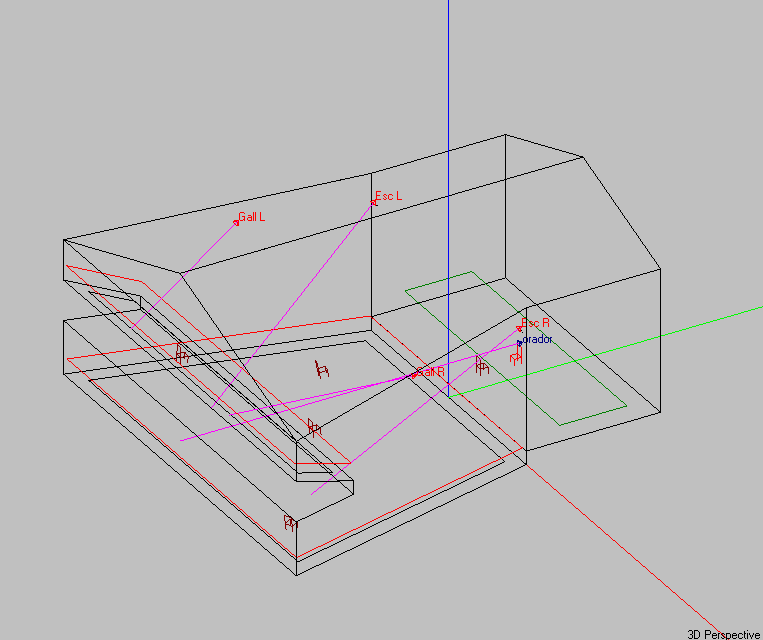
\includegraphics[width=\linewidth]{Para la memoria/Vista 3D.png}
        \caption{Vista 3D}
        \label{fig:3D}
    \end{subfigure}
    \begin{subfigure}[b]{0.45\linewidth}
        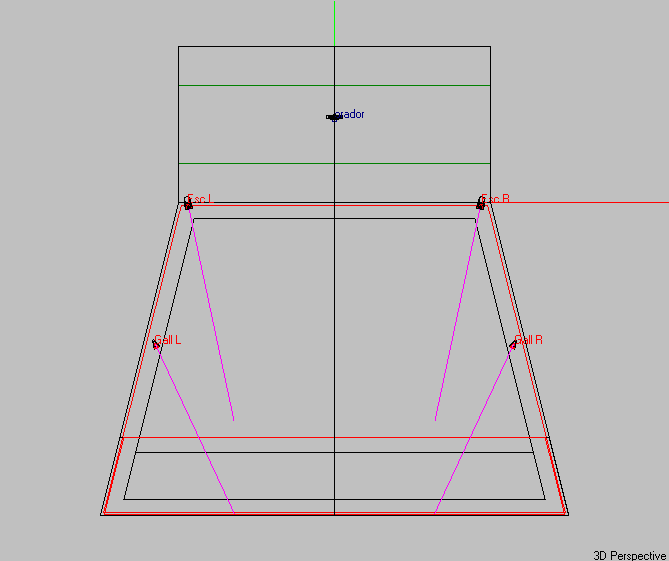
\includegraphics[width=\linewidth]{Para la memoria/Plano en planta.png}
        \caption{Planta}
        \label{fig:alzado}
    \end{subfigure}
    \begin{subfigure}[b]{0.45\linewidth}
        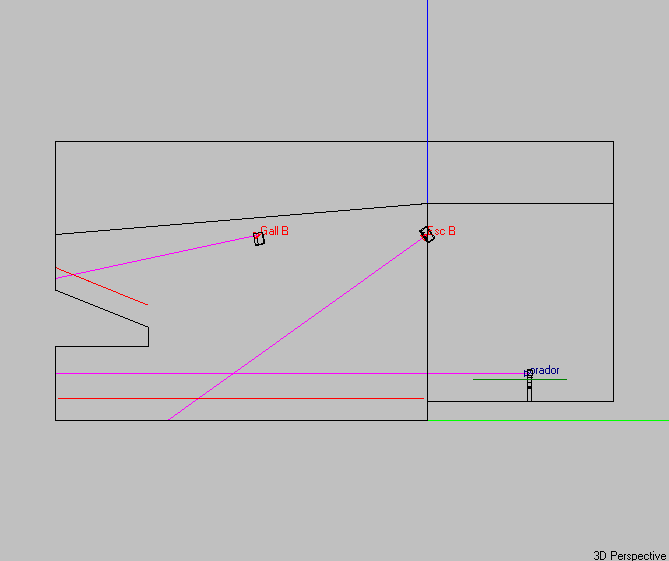
\includegraphics[width=\linewidth]{Para la memoria/Plano lateral.png}
        \caption{Perfil}
        \label{fig:perfil}
    \end{subfigure}
    \begin{subfigure}[b]{0.45\linewidth}
        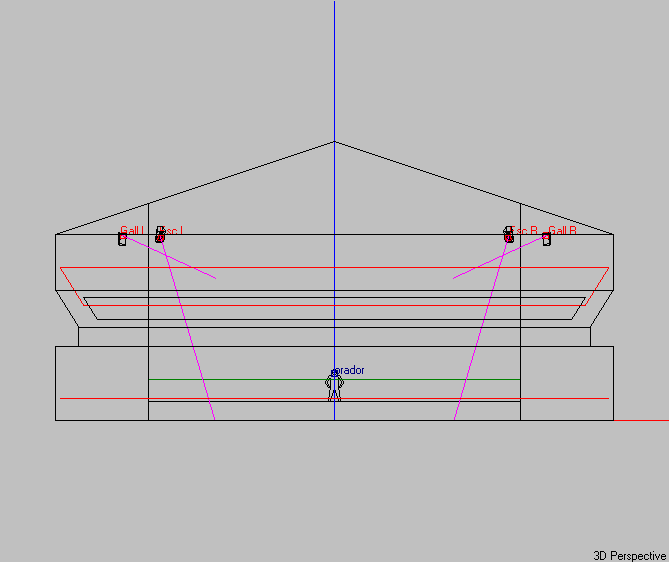
\includegraphics[width=\linewidth]{Para la memoria/Plano frontal.png}
        \caption{Alzado}
        \label{fig:alzado}
    \end{subfigure}
    \caption{Colocación de los altavoces en la sala}
    \label{fig:disposicion}
\end{figure}

\subsection{Ajuste de la uniformidad de campo directo a 1 kHz}

El requisito de uniformidad se cumple, ya que en la banda de \qty{1}{\kilo \hertz } la diferencia entre el nivel de presión sonora máximo y mínimo es menor a \qty{10}{\dB}. Concretamente, usando los datos de la \autoref{fig:uniformidad_dist_1k}:

\[ \Delta \text{SPL}_d = \text{SPL} _{\textnormal{máx}} - \text{SPL} _{\textnormal{mín}} = \qty{91.46}{\dB_{\text{SPL}}} - \qty{83.48}{\dB_{\text{SPL}}} = \boxed{\qty{7.98}{\dB}} < \qty{10}{\dB} \]

\begin{figure}[H]
    \centering
    \begin{subfigure}[b]{0.45\linewidth}
        \includegraphics[width=\linewidth]{Para la memoria/Ajuste de la uniformidad de campo directo a 1kHz - Distribución.png}
        \caption{Distribución del campo directo a \qty{1}{\kilo \hertz}}
        \label{fig:uniformidad_dist_1k}
    \end{subfigure}
    \begin{subfigure}[b]{0.45\linewidth}
        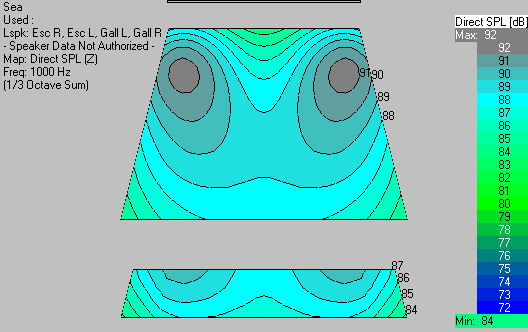
\includegraphics[width=\linewidth]{Para la memoria/Ajuste de la uniformidad de campo directo a 1kHz - Mapa.png}
        \caption{Mapa del campo directo a \qty{1}{\kilo \hertz}}
        \label{fig:uniformidad_mapa_1k}
    \end{subfigure}
    \begin{subfigure}[b]{0.45\linewidth}
        \includegraphics[width=\linewidth]{Para la memoria/Ajuste de la uniformidad de campo directo a 250 Hz - Distribución.png}
        \caption{Distribución del campo directo a \qty{250}{\hertz}}
        \label{fig:uniformidad_dist_250}
    \end{subfigure}
    \begin{subfigure}[b]{0.45\linewidth}
        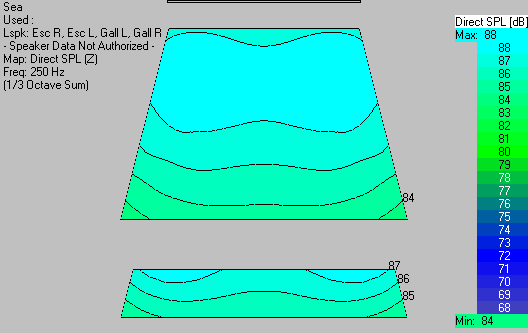
\includegraphics[width=\linewidth]{Para la memoria/Ajuste de la uniformidad de campo directo a 250 Hz - Mapa.png}
        \caption{Mapa del campo directo a \qty{250}{\hertz}}
        \label{fig:uniformidad_mapa_250}
    \end{subfigure}
    \begin{subfigure}[b]{0.45\linewidth}
        \includegraphics[width=\linewidth]{Para la memoria/Ajuste de la uniformidad de campo directo a 5kHz - Distribución.png}
        \caption{Distribución del campo directo a \qty{5}{\kilo \hertz}}
        \label{fig:uniformidad_dist_5k}
    \end{subfigure}
    \begin{subfigure}[b]{0.45\linewidth}
        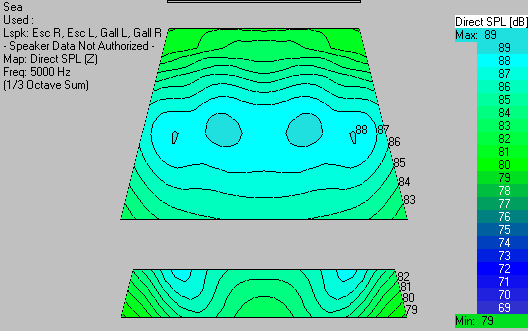
\includegraphics[width=\linewidth]{Para la memoria/Ajuste de la uniformidad de campo directo a 5kHz - Mapa.png}
        \caption{Mapa del campo directo a \qty{5}{\kilo \hertz}}
        \label{fig:uniformidad_mapa_5k}
    \end{subfigure}
    \caption{Representación de los niveles de presión sonora debidos a campo directo en la sala SEA para varias frecuencias significativas.}
    \label{fig:uniformidad_campo_directo}
\end{figure}

\subsection{Balance de potencia}

En la \autoref{tab:balance_potencias} aparecen representados los niveles de presión generada por cada altavoz. Si se quisiera obtener la potencia eléctrica que se debe suministrar a cada altavoz, habría que utilizar la sensibilidad aportada en las especificaciones. En total, Esc L y Esc R utilizan \qty{519}{\watt} cada uno, la vía de graves de Gall L y Gall R utiliza \qty{28}{\watt} y la vía de agudos de estos utiliza \qty{6.2}{\watt}.

% Table generated by Excel2LaTeX from sheet 'Loudspeakers'
\begin{table}[htbp]
    \centering
    \caption{Niveles SPL generados por cada altavoz a \qty{1}{\metre }, por bandas}
    \begin{tabular}{|c|r|r|r|r|}
        \hline
        \rowcolor[rgb]{ .439,  .678,  .278} \textcolor[rgb]{ 1,  1,  1}{\textbf{Frequency}} & \multicolumn{1}{c|}{\textcolor[rgb]{ 1,  1,  1}{\textbf{Esc L}}} & \multicolumn{1}{c|}{\textcolor[rgb]{ 1,  1,  1}{\textbf{Esc R}}} & \multicolumn{1}{c|}{\textcolor[rgb]{ 1,  1,  1}{\textbf{Gall L}}} & \multicolumn{1}{c|}{\textcolor[rgb]{ 1,  1,  1}{\textbf{Gall R}}} \bigstrut \\        \hline
        \rowcolor[rgb]{ .439,  .678,  .278} \textcolor[rgb]{ 1,  1,  1}{\textbf{100 Hz }}   & \cellcolor[rgb]{ 1,  1,  1}106.13                                & \cellcolor[rgb]{ .886,  .937,  .855}106.13                       & \cellcolor[rgb]{ 1,  1,  1}100.04                                 & \cellcolor[rgb]{ .886,  .937,  .855}100.04 \bigstrut                        \\        \hline
        \rowcolor[rgb]{ .439,  .678,  .278} \textcolor[rgb]{ 1,  1,  1}{\textbf{125 Hz }}   & \cellcolor[rgb]{ 1,  1,  1}105.78                                & \cellcolor[rgb]{ .886,  .937,  .855}105.78                       & \cellcolor[rgb]{ 1,  1,  1}99.69                                  & \cellcolor[rgb]{ .886,  .937,  .855}99.69 \bigstrut                         \\        \hline
        \rowcolor[rgb]{ .439,  .678,  .278} \textcolor[rgb]{ 1,  1,  1}{\textbf{160 Hz }}   & \cellcolor[rgb]{ 1,  1,  1}106.51                                & \cellcolor[rgb]{ .886,  .937,  .855}106.51                       & \cellcolor[rgb]{ 1,  1,  1}100.42                                 & \cellcolor[rgb]{ .886,  .937,  .855}100.42 \bigstrut                        \\        \hline
        \rowcolor[rgb]{ .439,  .678,  .278} \textcolor[rgb]{ 1,  1,  1}{\textbf{200 Hz }}   & \cellcolor[rgb]{ 1,  1,  1}107.37                                & \cellcolor[rgb]{ .886,  .937,  .855}107.37                       & \cellcolor[rgb]{ 1,  1,  1}101.28                                 & \cellcolor[rgb]{ .886,  .937,  .855}101.28 \bigstrut                        \\        \hline
        \rowcolor[rgb]{ .439,  .678,  .278} \textcolor[rgb]{ 1,  1,  1}{\textbf{250 Hz }}   & \cellcolor[rgb]{ 1,  1,  1}107.69                                & \cellcolor[rgb]{ .886,  .937,  .855}107.69                       & \cellcolor[rgb]{ 1,  1,  1}101.60                                 & \cellcolor[rgb]{ .886,  .937,  .855}101.60 \bigstrut                        \\        \hline
        \rowcolor[rgb]{ .439,  .678,  .278} \textcolor[rgb]{ 1,  1,  1}{\textbf{315 Hz }}   & \cellcolor[rgb]{ 1,  1,  1}108.27                                & \cellcolor[rgb]{ .886,  .937,  .855}108.27                       & \cellcolor[rgb]{ 1,  1,  1}102.18                                 & \cellcolor[rgb]{ .886,  .937,  .855}102.18 \bigstrut                        \\        \hline
        \rowcolor[rgb]{ .439,  .678,  .278} \textcolor[rgb]{ 1,  1,  1}{\textbf{400 Hz }}   & \cellcolor[rgb]{ 1,  1,  1}109.10                                & \cellcolor[rgb]{ .886,  .937,  .855}109.10                       & \cellcolor[rgb]{ 1,  1,  1}103.01                                 & \cellcolor[rgb]{ .886,  .937,  .855}103.01 \bigstrut                        \\        \hline
        \rowcolor[rgb]{ .439,  .678,  .278} \textcolor[rgb]{ 1,  1,  1}{\textbf{500 Hz }}   & \cellcolor[rgb]{ 1,  1,  1}108.54                                & \cellcolor[rgb]{ .886,  .937,  .855}108.54                       & \cellcolor[rgb]{ 1,  1,  1}102.45                                 & \cellcolor[rgb]{ .886,  .937,  .855}102.45 \bigstrut                        \\        \hline
        \rowcolor[rgb]{ .439,  .678,  .278} \textcolor[rgb]{ 1,  1,  1}{\textbf{630 Hz }}   & \cellcolor[rgb]{ 1,  1,  1}109.92                                & \cellcolor[rgb]{ .886,  .937,  .855}109.92                       & \cellcolor[rgb]{ 1,  1,  1}103.83                                 & \cellcolor[rgb]{ .886,  .937,  .855}103.83 \bigstrut                        \\        \hline
        \rowcolor[rgb]{ .439,  .678,  .278} \textcolor[rgb]{ 1,  1,  1}{\textbf{800 Hz }}   & \cellcolor[rgb]{ 1,  1,  1}110.48                                & \cellcolor[rgb]{ .886,  .937,  .855}110.48                       & \cellcolor[rgb]{ 1,  1,  1}104.39                                 & \cellcolor[rgb]{ .886,  .937,  .855}104.39 \bigstrut                        \\        \hline
        \rowcolor[rgb]{ .439,  .678,  .278} \textcolor[rgb]{ 1,  1,  1}{\textbf{1 kHz }}    & \cellcolor[rgb]{ 1,  1,  1}112.01                                & \cellcolor[rgb]{ .886,  .937,  .855}112.01                       & \cellcolor[rgb]{ 1,  1,  1}105.92                                 & \cellcolor[rgb]{ .886,  .937,  .855}105.92 \bigstrut                        \\        \hline
        \rowcolor[rgb]{ .439,  .678,  .278} \textcolor[rgb]{ 1,  1,  1}{\textbf{1.25 kHz }} & \cellcolor[rgb]{ 1,  1,  1}112.53                                & \cellcolor[rgb]{ .886,  .937,  .855}112.53                       & \cellcolor[rgb]{ 1,  1,  1}106.44                                 & \cellcolor[rgb]{ .886,  .937,  .855}106.44 \bigstrut                        \\        \hline
        \rowcolor[rgb]{ .439,  .678,  .278} \textcolor[rgb]{ 1,  1,  1}{\textbf{1.6 kHz }}  & \cellcolor[rgb]{ 1,  1,  1}114.53                                & \cellcolor[rgb]{ .886,  .937,  .855}114.53                       & \cellcolor[rgb]{ 1,  1,  1}108.44                                 & \cellcolor[rgb]{ .886,  .937,  .855}108.44 \bigstrut                        \\        \hline
        \rowcolor[rgb]{ .439,  .678,  .278} \textcolor[rgb]{ 1,  1,  1}{\textbf{2 kHz }}    & \cellcolor[rgb]{ 1,  1,  1}115.28                                & \cellcolor[rgb]{ .886,  .937,  .855}115.28                       & \cellcolor[rgb]{ 1,  1,  1}109.19                                 & \cellcolor[rgb]{ .886,  .937,  .855}109.19 \bigstrut                        \\        \hline
        \rowcolor[rgb]{ .439,  .678,  .278} \textcolor[rgb]{ 1,  1,  1}{\textbf{2.5 kHz }}  & \cellcolor[rgb]{ 1,  1,  1}113.81                                & \cellcolor[rgb]{ .886,  .937,  .855}113.81                       & \cellcolor[rgb]{ 1,  1,  1}107.72                                 & \cellcolor[rgb]{ .886,  .937,  .855}107.72 \bigstrut                        \\        \hline
        \rowcolor[rgb]{ .439,  .678,  .278} \textcolor[rgb]{ 1,  1,  1}{\textbf{3.15 kHz }} & \cellcolor[rgb]{ 1,  1,  1}112.64                                & \cellcolor[rgb]{ .886,  .937,  .855}112.64                       & \cellcolor[rgb]{ 1,  1,  1}106.55                                 & \cellcolor[rgb]{ .886,  .937,  .855}106.55 \bigstrut                        \\        \hline
        \rowcolor[rgb]{ .439,  .678,  .278} \textcolor[rgb]{ 1,  1,  1}{\textbf{4 kHz }}    & \cellcolor[rgb]{ 1,  1,  1}112.31                                & \cellcolor[rgb]{ .886,  .937,  .855}112.31                       & \cellcolor[rgb]{ 1,  1,  1}106.22                                 & \cellcolor[rgb]{ .886,  .937,  .855}106.22 \bigstrut                        \\        \hline
        \rowcolor[rgb]{ .439,  .678,  .278} \textcolor[rgb]{ 1,  1,  1}{\textbf{5 kHz }}    & \cellcolor[rgb]{ 1,  1,  1}111.21                                & \cellcolor[rgb]{ .886,  .937,  .855}111.21                       & \cellcolor[rgb]{ 1,  1,  1}105.12                                 & \cellcolor[rgb]{ .886,  .937,  .855}105.12 \bigstrut                        \\        \hline
        \rowcolor[rgb]{ .439,  .678,  .278} \textcolor[rgb]{ 1,  1,  1}{\textbf{6.3 kHz }}  & \cellcolor[rgb]{ 1,  1,  1}111.13                                & \cellcolor[rgb]{ .886,  .937,  .855}111.13                       & \cellcolor[rgb]{ 1,  1,  1}105.04                                 & \cellcolor[rgb]{ .886,  .937,  .855}105.04 \bigstrut                        \\        \hline
        \rowcolor[rgb]{ .439,  .678,  .278} \textcolor[rgb]{ 1,  1,  1}{\textbf{8 kHz }}    & \cellcolor[rgb]{ 1,  1,  1}110.22                                & \cellcolor[rgb]{ .886,  .937,  .855}110.22                       & \cellcolor[rgb]{ 1,  1,  1}104.13                                 & \cellcolor[rgb]{ .886,  .937,  .855}104.13 \bigstrut                        \\        \hline
        \rowcolor[rgb]{ .439,  .678,  .278} \textcolor[rgb]{ 1,  1,  1}{\textbf{10 kHz }}   & \cellcolor[rgb]{ 1,  1,  1}110.17                                & \cellcolor[rgb]{ .886,  .937,  .855}110.17                       & \cellcolor[rgb]{ 1,  1,  1}104.08                                 & \cellcolor[rgb]{ .886,  .937,  .855}104.08 \bigstrut                        \\        \hline
    \end{tabular}%
    \label{tab:balance_potencias}%
\end{table}%


\subsection{Ecualización. Niveles promedio de banda ancha con y sin ponderación A}

En la \autoref{fig:EQ} aparecen las curvas resultantes de la ecualización (cálculos adjuntos en el documento de Excel). En la \autoref{fig:EQ_2} aparecen las respuestas en frecuencia en cada punto de escucha por bandas.

\begin{figure}[hbtp]
    \centering
    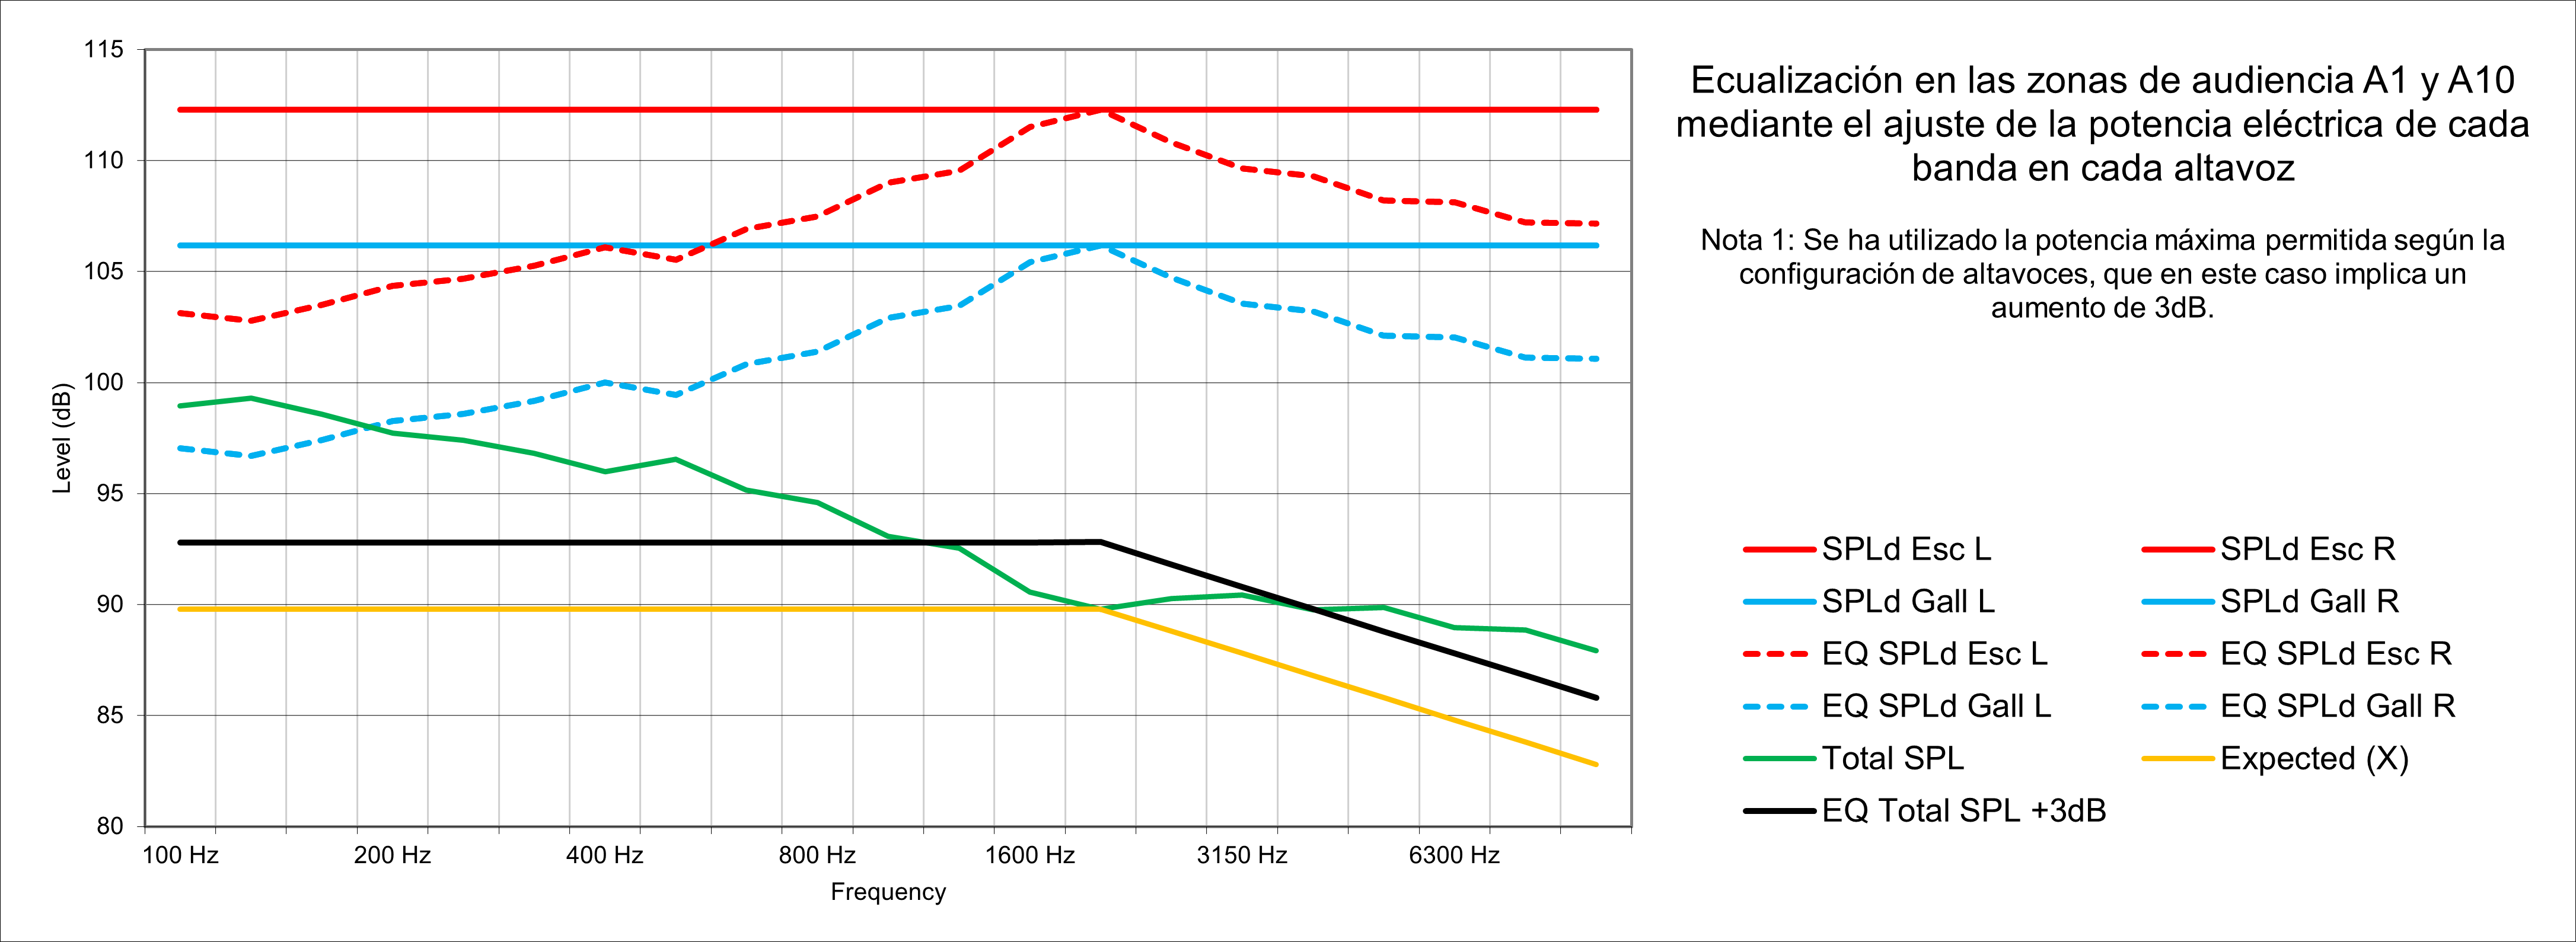
\includegraphics[width=\linewidth]{Para la memoria/EQ.png}
    \caption{Curvas de ecualización}
    \label{fig:EQ}
\end{figure}

\begin{figure}[hbtp]
    \centering
    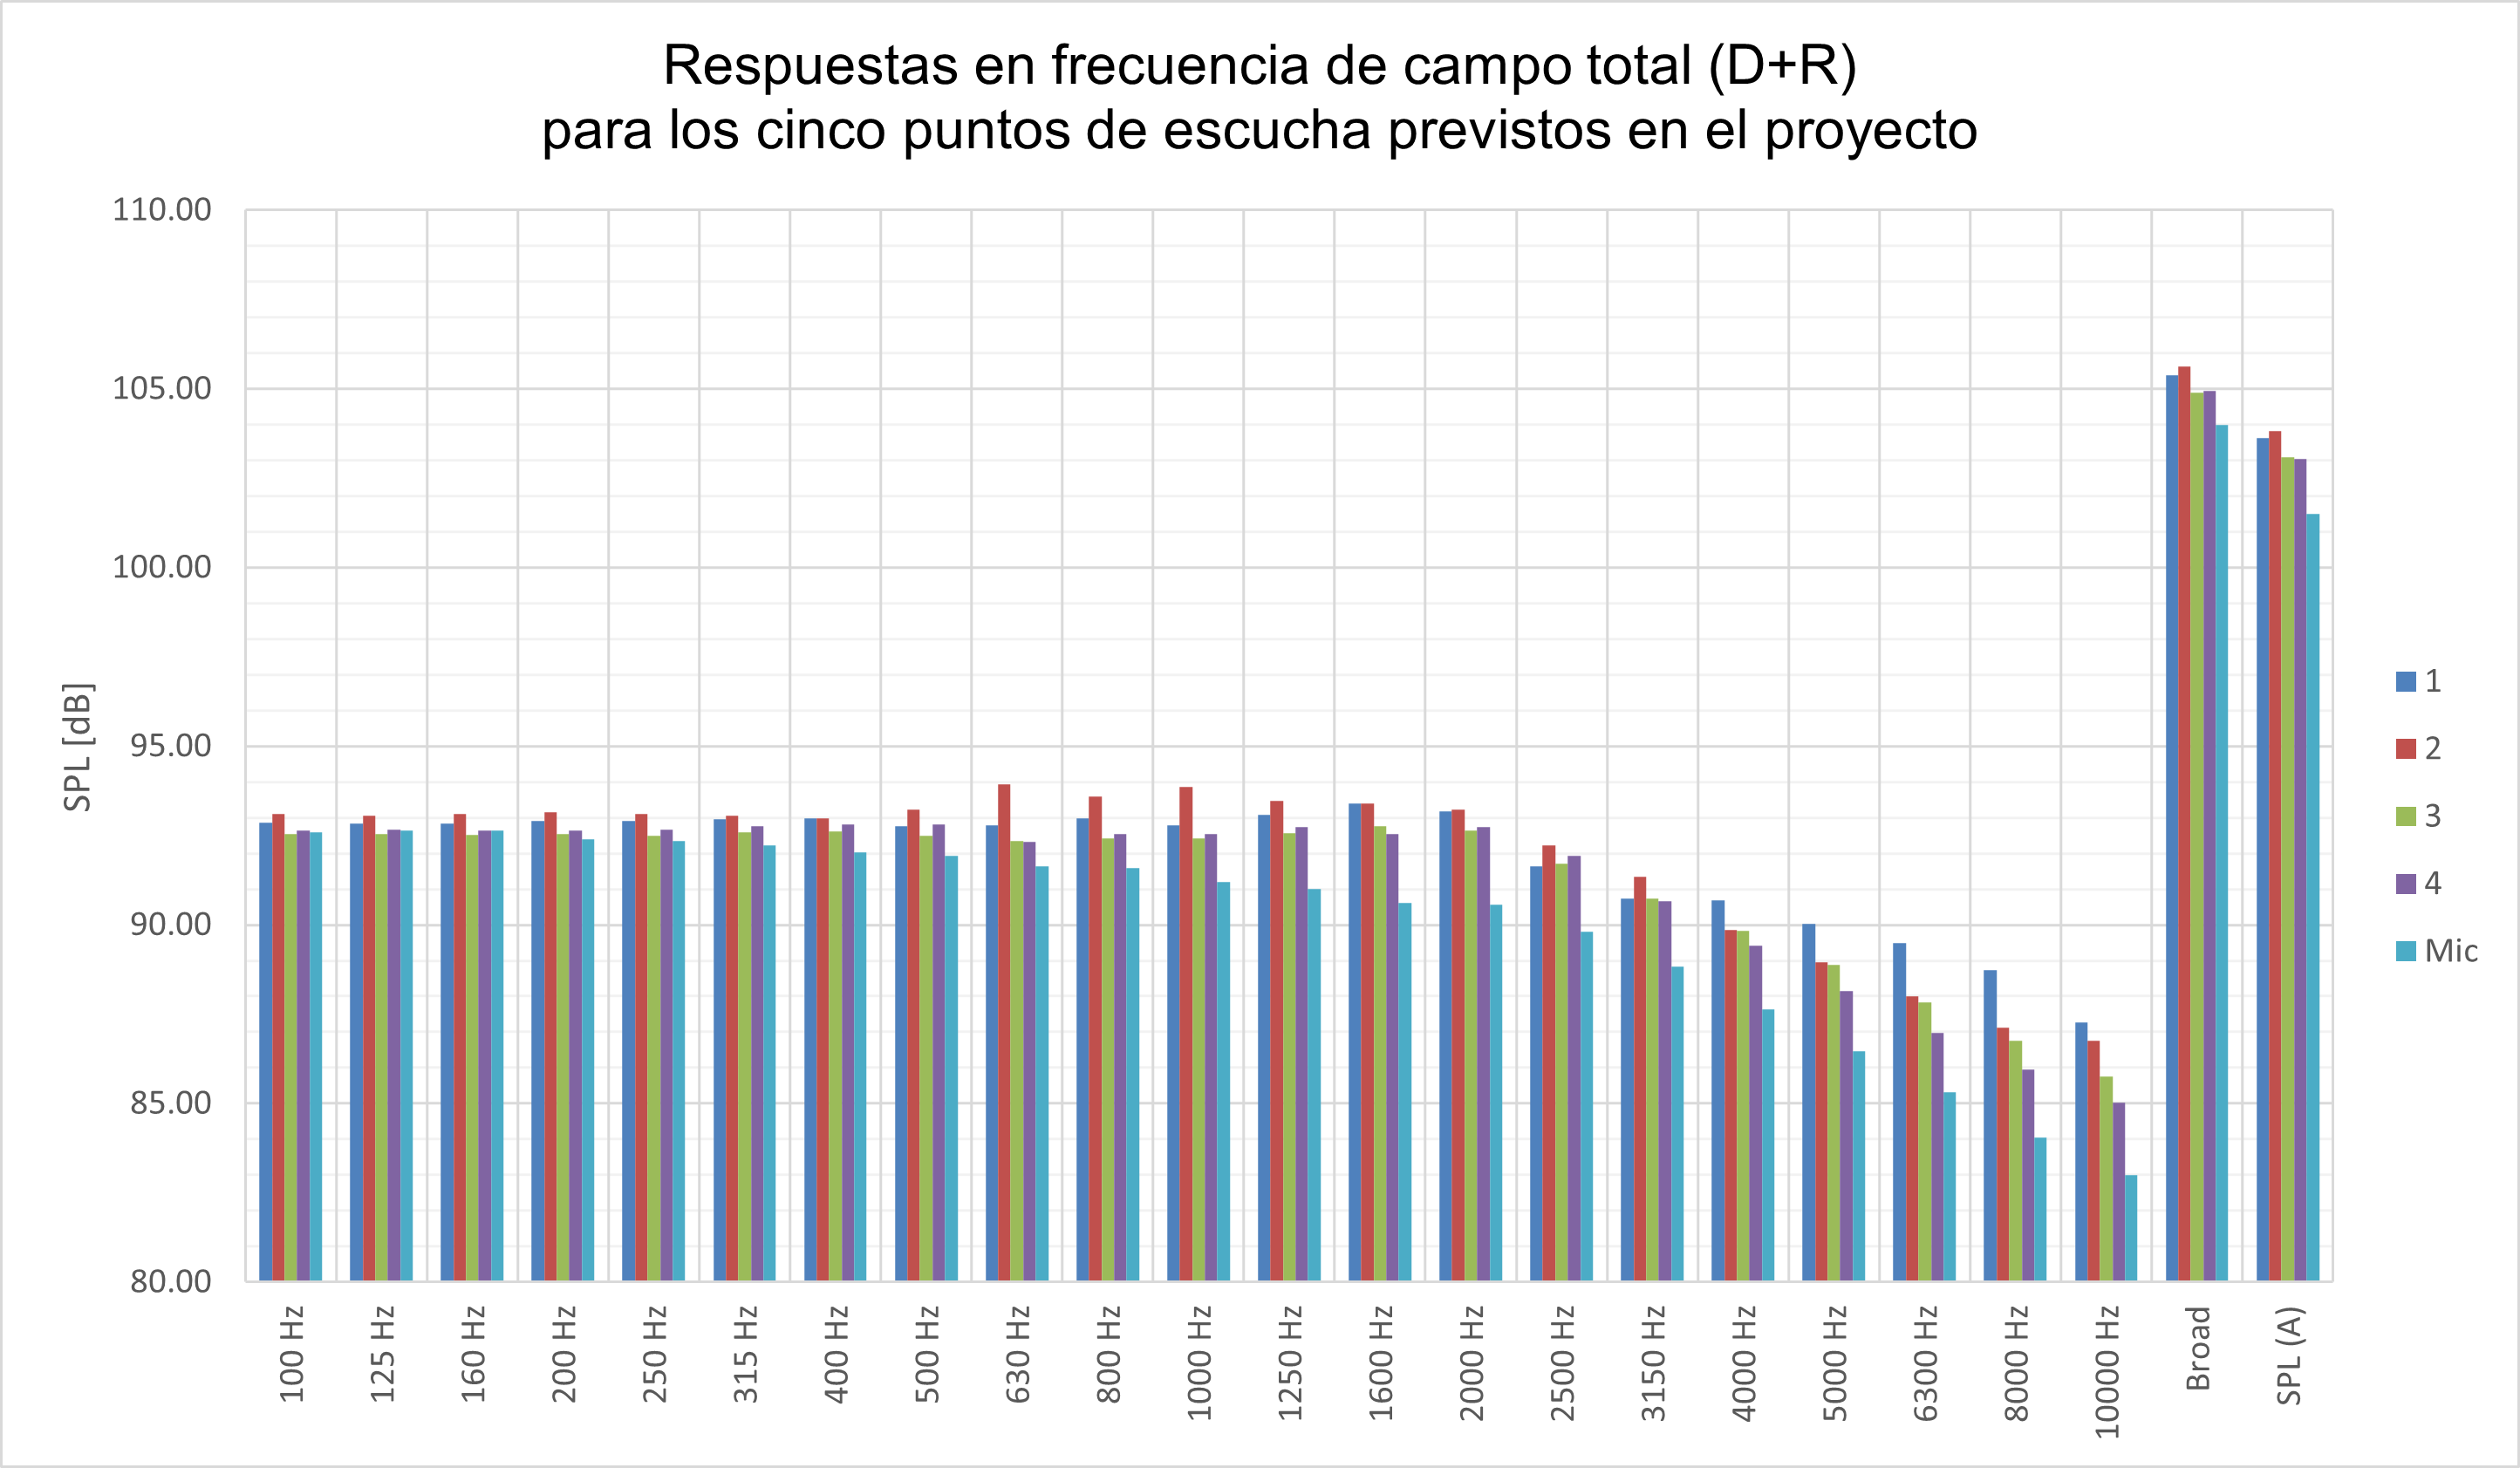
\includegraphics[width=\linewidth]{Para la memoria/EQ 2.png}
    \caption{Respuesta en frecuencia en cada punto de escucha por bandas}
    \label{fig:EQ_2}
\end{figure}


\subsection{Retardos}

En la \autoref{tab:colocacion_altavoces} aparecen los diferentes retardos que se han aplicado a cada altavoz. En la \autoref{fig:retardos} el mapa de \textit{Arrival Time}.

\begin{figure}[hbtp]
    \centering
    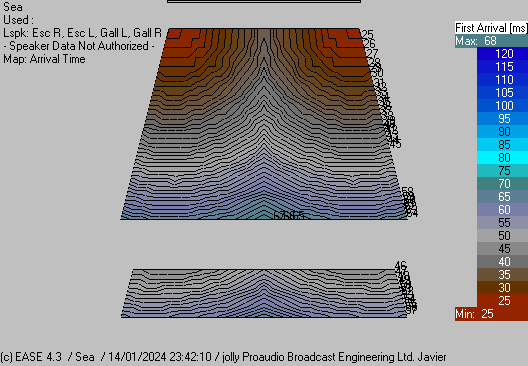
\includegraphics[width=0.7\linewidth]{Para la memoria/Arrival time AURA.png}
    \caption{Mapa de Arrival Time calculado con AURA}
    \label{fig:retardos}
\end{figure}

\subsection{Inteligibilidad}

\begin{figure}
    \centering
    \includegraphics[width=\linewidth]{Para la memoria/Inteligibilidad - STD Mapping - STI - Distribución.png}
    \caption{Distribución de STI mediante Standard Mapping}
    \label{fig:STI}
\end{figure}
\begin{figure}
    \centering
    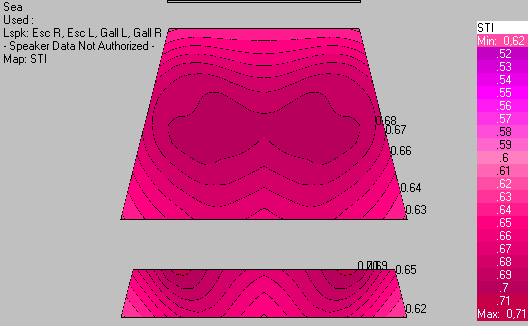
\includegraphics[width=\linewidth]{Para la memoria/Inteligibilidad - STD Mapping - STI - Mapa.png}
    \caption{Mapa de STI mediante Standard Mapping}
    \label{fig:STI}
\end{figure}

%\nocite{*}
%\newpage
%\bibliography{Bibliography}
%\bibliographystyle{babplain}


\newpage
\appendix
\section{Especificaciones técnicas de los altavoces} \label{app:specs}

En las siguientes páginas se incluyen las especificaciones de los altavoces utilizados en este proyecto.

% Inserta un PDF
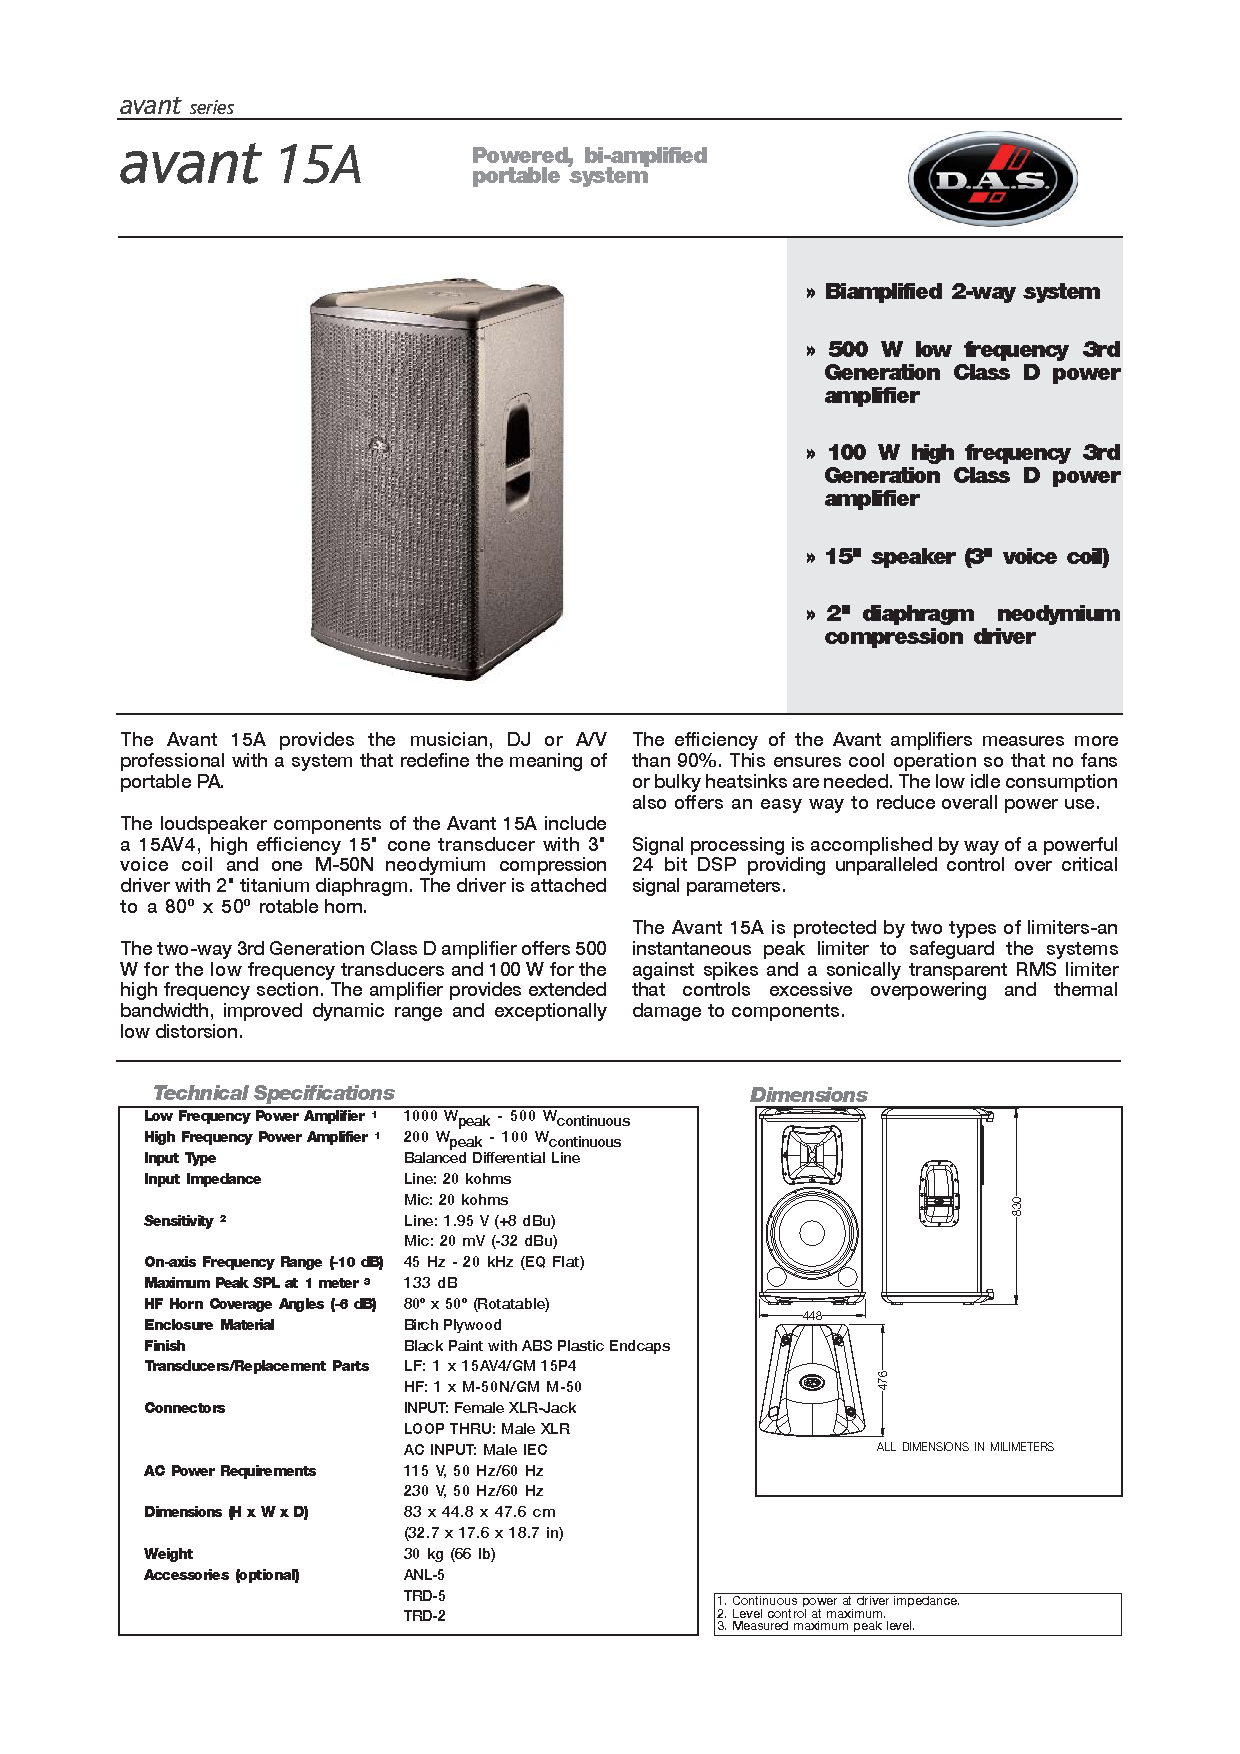
\includepdf[pages=-]{Para la memoria/Specs Avant 15A.pdf}

\includepdf[pages=4-4]{Para la memoria/Specs TRAP JR - 6K.pdf}

\end{document}
